% Copyright 2021 Edoardo Riggio

% Licensed under the Apache License, Version 2.0 (the "License");
% you may not use this file except in compliance with the License.
% You may obtain a copy of the License at

% 	http://www.apache.org/licenses/LICENSE-2.0

% Unless required by applicable law or agreed to in writing, software
% distributed under the License is distributed on an "AS IS" BASIS,
% WITHOUT WARRANTIES OR CONDITIONS OF ANY KIND, either express or implied.
% See the License for the specific language governing permissions and
% limitations under the License.

\documentclass{article}

\usepackage{amsmath, graphicx, hyperref}
\usepackage{fancyvrb, newverbs, xcolor}

\definecolor{cverbbg}{gray}{0.93}

\newenvironment{cverbatim}
 {\SaveVerbatim{cverb}}
 {\endSaveVerbatim
  \flushleft\fboxrule=0pt\fboxsep=.5em
  \colorbox{cverbbg}{\BUseVerbatim{cverb}}%
  \endflushleft
}

\newenvironment{lcverbatim}
 {\SaveVerbatim{cverb}}
 {\endSaveVerbatim
  \flushleft\fboxrule=0pt\fboxsep=.5em
  \colorbox{cverbbg}{%
    \makebox[\dimexpr\linewidth-2\fboxsep][l]{\BUseVerbatim{cverb}}%
  }
  \endflushleft
}

\newcommand{\ctexttt}[1]{\colorbox{cverbbg}{\texttt{#1}}}
\newverbcommand{\cverb}
  {\setbox\verbbox\hbox\bgroup}
  {\egroup\colorbox{cverbbg}{\box\verbbox}}

\begin{document}
\begin{titlepage}
    \begin{center}
        \vspace*{1cm}
        
        \Huge
        \textbf{Data Management Cheatsheet}
        
        \vspace{0.5cm}
        \LARGE
        
        \vspace{.5cm}
        
        Edoardo Riggio
   		  \vspace{1.5cm}
       
        \vfill
        
        \today
        
        \vspace{.8cm}
          \Large
          Data Management - SP. 2021 \\
        Computer Science\\
        Universit\`{a} della Svizzera Italiana, Lugano\\
        
    \end{center}
\end{titlepage}

\tableofcontents

\newpage

\section{Entity Relationship Models}
\subsection{Purpose}
Provides a common, informal, and convenient method for communication between application end users and the database designers to model the information's structure. \\ \\
The ER model frequently employs \textbf{ER diagrams}, which are graphic descriptions to visualize the information's structure.

\subsection{Basic Concepts}
The three basic concepts are:
\subsubsection{Entity}
It is an "object". All entities of the same "type" form an \textbf{entity set}. \\ \\
Pictorially, it is denoted by a rectangle, with its typewritten inside. It must be a singular noun and capitalized (all capitals for acronyms). \\ \\

\centerline{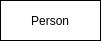
\includegraphics[width=2cm]{./assets/entity.png}}
	
\subsubsection{Attribute}
An entity can have a set of zero or more attributes, which are some properties. All entities in the entity set have the same properties, though not generally with the same values. \\ \\
Pictorially, attributes of an entity are written in ellipses connected to the entity. \\ \\ \\

\centerline{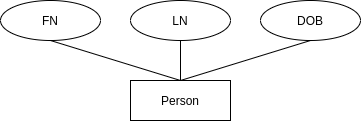
\includegraphics[width=7.5cm]{./assets/attribute.png}}
\vspace{.6cm}
\noindent Attributes can be of several different types:

\begin{itemize}
	\item \textbf{Base}
	
	\item \textbf{Simple}
	
	\item \textbf{Single-valued}
	
	\item \textbf{Derived}
	\vspace{.2cm} \\
	An attribute whose value is derived from other factors (e.g., age from DOB and the current date). \\ \\
	
	\centerline{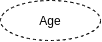
\includegraphics[width=2cm]{./assets/derived.png}}
	
	\item \textbf{Composite}
	\vspace{.2cm} \\
	An attribute that has multiple component attributes attached to it. \\ \\
	
	\centerline{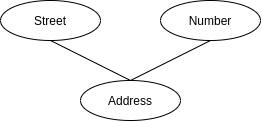
\includegraphics[width=5.2cm]{./assets/composite.png}}
	
	\item \textbf{Multi-valued}
	\vspace{.2cm} \\
	An unspecified number of values in this type of attribute. \\ \\
	
	\centerline{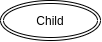
\includegraphics[width=2cm]{./assets/multivalued.png}}
\end{itemize}
	
\subsubsection{Relationship}
Several entity sets can participate in a relationship.\\ \\
Pictorially, a relationship is defined as a diamond with a verb inside. This verb should be in third person singular and capitalized. \\ \\
Relationships can be:

\begin{itemize}
	\item \textbf{Binary}
	\vspace{.2cm} \\
	A binary relationship can be \textbf{many-to-one} iff for each element of A, there exists at most one element of B related to it (e.g., the relationship "born" between a person and a country). \\ \\
	
	\centerline{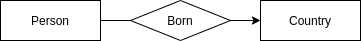
\includegraphics[width=7cm]{./assets/many-to-one.png}}
	\vspace{.6cm}
	A binary relationship can be \textbf{one-to-one} iff for each element of A, there exists at most one element of B related to it, and for each element of B, there exists at most one element of A related to it (e.g., the relationship "heads" between a person and a country). \\ \\
	
	\centerline{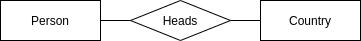
\includegraphics[width=7cm]{./assets/one-to-one.png}}
	\vspace{.6cm}
	A binary relationship can be \textbf{many-to-many} if it is not many-to-one from A to B, and it is not many-to-one from B to A (e.g., the relationship "likes" between a person and a country). \\ \\
	
	\centerline{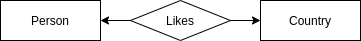
\includegraphics[width=7cm]{./assets/many-to-many.png}}
	\vspace{.6cm}
	
	\item \textbf{Ternary}
	\vspace{.2cm} \\
	This relationship is between three distinct entity relationships. \\ \\
	
	\centerline{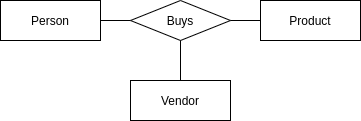
\includegraphics[width=7cm]{./assets/ternary.png}}
	\vspace{.6cm}
	
	\item \textbf{Non-Distinct Entity Set}
	\vspace{.2cm} \\
	In this case, it is frequently useful to give roles to the participating entities. \\ \\
	
	\centerline{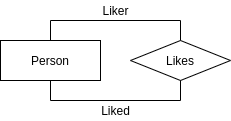
\includegraphics[width=4.5cm]{./assets/nondistinct.png}}
	\vspace{.6cm}
\end{itemize}

\subsection{Keys}
Some subset of the attributes of an entity has the property that two different entities in an entity set must \textbf{differ on the values of the attributes}. Such a set of attributes is called a \textbf{superkey}. A minimal superkey is called a \textbf{key} (also called a \textbf{candidate key}).

\subsubsection{Primary Keys}
If an entity has one or more keys, then one of them is chosen as the \textbf{primary key}. \\ \\

\centerline{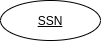
\includegraphics[width=2cm]{./assets/key.png}}

\subsection{Relationships as Entities}
Considering relationships as entities allows us to let relationships participate in other "high order" relationships. \\ \\ \\

\centerline{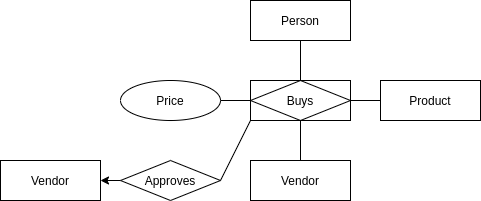
\includegraphics[width=9cm]{./assets/rel-ent.png}}
\vspace{.6cm}

\subsection{Strong and Weak Entities}
The elements of a \textbf{strong entity set} can be identified by the values of their attributes. That is, it has a primary key made of its attributes. \\ \\
The elements of a \textbf{weak entity set} cannot be identified by the values of their attributes. There is no primary key made from its attributes. \\ \\
In the case below, a Man can only be identified by the combination of the Woman to whom he is related and his Name -- which is now a \textbf{discriminant}. \\ \\ \\

\centerline{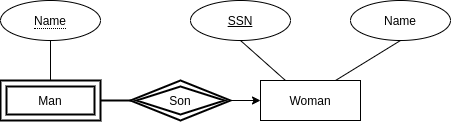
\includegraphics[width=8cm]{./assets/weak.png}}
\vspace{.6cm}

\subsection{ISA Relationships}
The subset relationship between the set and its subset is called ISA. The elements of the subset all have the same attributes and relationships as the set elements. In addition, they may participate in relationships and have attributes that make sense to them. \\ \\
The elements of the subset are \textbf{weak entities}. \\ \\ \\

\centerline{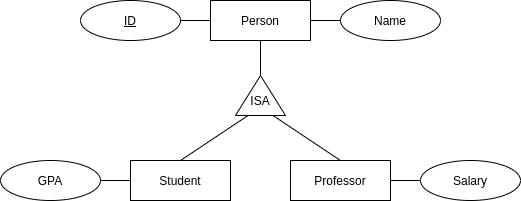
\includegraphics[width=9.5cm]{./assets/isa.png}}
\vspace{.6cm}

\begin{itemize}
	\item \textbf{Disjoint}
	\vspace{.2cm} \\
	No Entity could be in more than one subclass.
	
	\item \textbf{Overlapping}
	\vspace{.2cm} \\
	An Entity could be in more than one subclass.
	
	\item \textbf{Total}
	\vspace{.2cm} \\
	Every Entity has to be in at least one subclass.
	
	\item \textbf{Partial}
	\vspace{.2cm} \\
	An Entity does not have to be in any subclass.
\end{itemize}

\subsection{Cardinality Constraints}
It is possible to specify how many times each entity from some entity set can participate in some relationship. Constraint can be specified as:

\begin{itemize}
	\item \textbf{0..*}
	\vspace{.2cm} \\
	This means there are no constraints.
	
	\item \textbf{i..i}
	\vspace{.2cm} \\
	Means that the constraint must be exactly $i$.
	
	\item \textbf{i..j}
	\vspace{.2cm} \\
	Means that the constraints can go from $i$ up to $j$.
\end{itemize}
Constraints are \textbf{look across}, meaning that in the following example:

\begin{itemize}
	\item Every person likes exactly 1 country
	\item Every country is liked by 2 or 3 people
\end{itemize}

\vspace{.6cm}
\centerline{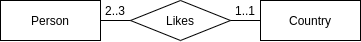
\includegraphics[width=7cm]{./assets/look-across.png}}
\vspace{.2cm}

\section{Relational Model}
\subsection{Sets}
A set is a "bag" of elements, some or all of which could be setting themselves. It is not possible to specify \textbf{how many times} or \textbf{in which position} does an element appear in a set.

\subsection{Relations}
Relations are elements such as \textbf{primary keys}, \textbf{keys}, \textbf{foreign keys}...

\subsubsection{Keys and Super keys}
A set of columns in a relation is a \textbf{superkey} iff any two tuples that are equal on the elements of these columns are completely equal. A relation always has \textbf{at least one} superkey. The set of all the attributes is a superkey. \\ \\
A minimal superkey is a \textbf{key}. A relation always has at least one key (but there could be more than one). Precisely one key is chosen as the \textbf{primary key}.

\subsubsection{Foreign Keys}
A foreign key is a column or group of columns in a relational database table that provides a link between data in two tables. It must always refer to a primary key somewhere in the database.

\subsection{Crow's Feet}
Crows' Feet are used to indicate constraint. The following are the possible Crow's Feet: \\ \\

\centerline{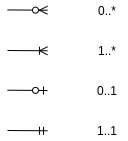
\includegraphics[width=3cm]{./assets/crows.png}}

\section{Normalization}
\subsection{Natural Join}
The natural join is a Cartesian join with the condition of equality on corresponding columns. Only one copy of each column is left.

\subsection{Lossless Join Decomposition}
This is another term for information not to be lost; we can reconstruct the original table by combining data from the two new tables using a natural join.

\subsection{Normalization}
Normalization involves reorganizing a relational database by breaking up tables to remove various anomalies.

\subsection{Normal Forms}
A standard form applies to a table/relation schema, not the whole database schema.

\subsubsection{1NF (First Normal Form)}
In 1NF, we have a relation; this means that there are no repeating groups and that the number of columns is fixed.

\subsubsection{2NF (Second Normal Form)}
2NF means that the table is in 1NF, and there are no \textbf{partial dependencies}.

\subsubsection{3NF (Third Normal Form)}
3NF means that the table is in 2NF, and there are no \textbf{transitive dependencies}.

\subsubsection{BCNF (Boyce-Codd Normal Form)}
BCNF means that the table is in 1NF, and every functional dependency is from a complete key. A table in BCNF is automatically a table in 3NF.

\subsection{Functional Dependencies}
The database rules can be described using functional dependencies. Let P and Q be sets of columns, then P functionally determines Q:

\[ P \rightarrow Q \]
If any two rows that are equal on P must be equal on Q. \\ \\
There are several types of keys:

\begin{itemize}
	\item \textbf{From the full key}
	
	\item \textbf{Not from the full key}
	\begin{itemize}
		\item \textbf{Partial Dependency}
		\vspace{.2cm} \\
		From a part of the primary key to outside the key.
		
		\item \textbf{Transitive Dependency}
		\vspace{.2cm} \\
		From outside the key to outside the key.
		
		\item \textbf{Into key dependency}
		\vspace{.2cm} \\
		From outside the key into (all or part of) the key.
	\end{itemize}
\end{itemize}
A set of attributes is a \textbf{key} iff $X^+ = R$ (meaning that the key $X$ is composed of all attributes $R$).

\subsection{Finding Keys}
In order to find all of the possible keys, we can divide the attributes into four distinct classes:

\begin{enumerate}
	\item \textbf{Appearing on both sides of FDs}
	\item \textbf{Appearing on left sides of FDs only}
	\item \textbf{Appearing on right sides of FDs only}
	\item \textbf{Not appearing in FDs}
\end{enumerate}
Staring from attributes in classes 2 and 4, add as many attributes in class 1 as needed. Ignore the attributes in class 3.

\subsection{Minimal Cover}
It is needed in order to simplify the set of FDs. It is done by following these steps:

\begin{enumerate}
	\item \textbf{Combine right hand sides}
	\vspace{.2cm} \\
	If the left-hand sides of the two FDs are the same, they can be merged into one FD.
	
	\item \textbf{Right-hand side simplification}
	
	\item \textbf{Left hand side simplification}
\end{enumerate}

\subsection{Create Tables}
In order to create the tables of the database, we need to follow these steps:

\begin{enumerate}
	\item \textbf{Get a minimal cover of the FDs}
	\item \textbf{Create tables from the minimal cover}
	\item \textbf{Remove redundant tables}
	\item \textbf{Ensure the storage of the global key}
	\vspace{.2cm} \\
	We need to check if one of the tables already contains the global key. If none have the global key, it is stored in another table.
\end{enumerate}

\subsection{Data Structures}
\subsubsection{Heap}
Assuming continuous storage, time complexities for \textbf{finding} elements are:

\[ O(1)~\text{or}~O(n) \] \\
It takes $O(1)$ in the case we are searching the head or tail (assuming both of them are accessible in
time $O(1)$) of the heap. It takes $O(n)$ if we try to find any element in the heap. \\ \\
Time complexities for \textbf{deleting} elements are:

\[ O(1)~\text{or}~O(n) \] \\
It takes $O(1)$ in the case we are deleting the head or tail (assuming both of them are accessible in
time $O(1)$) of the heap, and there is no memory compacting. It takes $O(n)$ if we try to delete an element accessible in 1, and there is memory compacting. \\ \\
Time complexities for \textbf{inserting} elements are:

\[ O(1)~\text{or}~O(n) \] \\
It takes $O(1)$ to insert an element in the front or back of the heap (if it is accessible in $O(1)$). It takes $O(n)$ if the end of the heap cannot be accessed in constant time.

\subsubsection{Sorted Sequence}
Time complexity for \textbf{finding} an element is:

\[ O(\log(n)) \] \\
It takes $O(log(n))$ to find an element in the sorted sequence. This is because binary search is used. \\ \\
Time complexities for \textbf{deleting} elements are:

\[ O(\log(n))~\text{or}~O(\log(n) + n) \] \\
It takes $O(\log(n))$ to delete the element because binary search is used, and there is no memory compacting. Since the time of binary search is $O(\log(n))$, and $O(1)$ to remove the found element, the total complexity is $O(\log(n))$. Deleting an element from a sorted sequence takes $O(\log(n) + n)$ when removing any element which is neither the head nor the tail of the sequence (assuming both of them are accessible in constant time). To delete the element in the sequence, it would take $\log(n)$ to find the element (assuming we are using some binary search algorithm), $O(1)$ to delete the element, and then $O(n)$ to compact the memory. \\ \\
Time complexities for \textbf{inserting} elements are:

\[ O(\log(n))~\text{or}~O(\log(n) + n) \] \\
If no compacting is used, it takes $O(\log(n))$ to insert an item. In this case, the time is used to search the space, and constant time is used to insert the element. It takes $O(\log(n) + n)$ if there is memory compacting. In this case, $O(\log(n))$ is used to find the space, constant time to insert the element, and $O(n)$ to recompact memory.

\subsubsection{Hashing}
Hashing is used in the following cases:

\begin{itemize}
	\item If the set of integers is large
	\item If many of the queries are not range queries
\end{itemize}

\subsubsection{B+ Tree}
B+ tree is used in the following cases:

\begin{itemize}
	\item If the set of integers is large
	\item If many of the queries are range queries
\end{itemize}
In order to computer the maximum number of nodes an internal node can have, we can use the following formula:

\[ m \cdot (P) + (m-1) \cdot (K) \leq B \] \\
Where \textbf{P} is the size of the pointer, \textbf{K} is the size of the key, and \textbf{B} is the size of the block (number of sectors). \\ \\
Given $m$, we know that the number of children of the \textbf{root} is between 2 and $m$, while the number of children of an \textbf{internal node} is between $\left\lceil\frac{m}{2}\right\rceil$ and $m$.

\subsection{Indexes}
\subsubsection{Dense Index}
An index is dense if, for every key appearing in (some record) of the data file, a dedicated pointer to the block containing the record appears in (some record) of the index file.

\subsubsection{Sparse Index}
An index is sparse if for not every key appearing in (some record) of the data file, a dedicated pointer to the block containing the record appears in (some record) of the index file.

\subsection{Files}
\subsubsection{Clustered File}
In a clustered file, blocks are composed of elements that are "close to" in memory -- as if the files were first sorted and then dispersed in memory.

\subsubsection{Unclustered Files}
Blocks are composed of elements that are not "close to" in memory in an unclustered file.

\subsection{External Merge Sort}
In order to compute the number of passes of the external merge sort, we use the following formula:

\[ N_P = 1 + \left\lceil \log_{B-1}\left(\frac{N}{B}\right) \right\rceil \] \\
Where \textbf{B} is the number of RAM blocks, and \textbf{N} is the number of blocks to sort. \\ \\
From the number of passes we can compute the cost as:

\[ C = (2 \cdot N) \cdot N_P \] \\
Where \textbf{N} is the number of blocks to sort, and $N_P$ is the number of passes.

\section{Transaction Processing - Recovery}
A \textbf{transaction} is an execution of a user's program.

\subsection{ACID Theorem}
A transaction is supposed to satisfy the \textbf{ACID} conditions. These conditions are:

\begin{itemize}
	\item \textbf{Atomic}
	\vspace{.2cm} \\
	It is not divisible into smaller units of executions. A transaction is either executed entirely or not executed at all.
	
	\item \textbf{Consistent}
	\vspace{.2cm} \\
	It preserves the consistency of the database. If started on a correct database and finished successfully, it will leave a correct database.
	
	\item \textbf{Isolated}
	\vspace{.2cm} \\
	A transaction is given the illusion of running on a dedicated system, so concurrency errors cannot be introduced. Transactions do not interact with one another.
	
	\item \textbf{Durable}
	\vspace{.2cm} \\
	Once completed correctly, the transaction's values will never be forgotten -- written to the database disk.
\end{itemize}

\subsection{Recovery}
The job of recovery is to make sure that the transaction satisfies \textbf{ACD} properties -- as \textbf{I} is not relevant in this case. \\ \\
If a failure occurred while a transaction was executing, we could not continue, and therefore we needed to \textbf{restore the database} to the state before the failed transaction started. \\ \\
If a failure occurred after a transaction finished executing, the state must \textbf{continue reflecting} this transaction. \\ \\
A history is \textbf{recoverable} if, for every transaction, $T$ that commits, the commit of T follows the commit of every transaction from which $T$ read.

\subsection{Cascading Aborts}
A history \textbf{avoids cascading aborts} if every transaction reads only values produced by transactions that have already been committed. \\ \\
\centerline{No Cascading Aborts = Recoverable}

\subsection{Strict Histories}
History is said to be \textbf{strict} if it satisfies the condition for avoiding cascading aborts, and -- for every transaction that writes an item -- all the transactions that previously wrote that item have already committed or aborted. \\ \\
\centerline{Strict = No Cascading Aborts}

\subsection{Checkpointing}
This technique is used to prevent the need to look at the complete log and thus reduce the work during recovery. \\ \\
During normal execution, the following steps are followed to the checkpoint:

\begin{enumerate}
	\item Stop processing
	\item Force the log buffers on the disk log
	\item Force the database buffers on the database disk
	\item Write onto the log a list of the transactions currently running
	\item Write "CHECKPOINT DONE" onto the log
	\item Resume processing
\end{enumerate}
Checkpointing synchronizes the database with the log.

\subsection{Recovery with Checkpointing}
To recover after a crash, we start by scanning the log \textbf{backward} until you reach the first checkpoint. You have two empty lists: the undo and the redo list. \\ \\
For every transaction that has a commit record, it is added to the redo list. Each transaction with a start record but no commit record is added to the undo list. Finally, for each transaction listed in the checkpoint record for which there is no commit record, it is added to the undo list. \\ \\
All of the transactions in the undo list are undone, and all the transactions in the redo list are redone.

\section{Transaction Processing - Concurrency}
\subsection{Concurrency}
Concurrency does \textbf{I} while possibly supporting \textbf{ACD}. Each transaction should run as if there were no other transactions in the system. \\ \\
A \textbf{history} is a trace of the behavior of a set of transactions, listing the reads and writes in order of execution.

\subsection{Serial Histories}
A history is \textbf{serial} if it describes a serial execution, meaning that transactions follow each other -- without concurrency. A concurrent execution that happens to be serial is a correct concurrent execution.

\subsection{Serializable Histories}
A history H is said to be \textbf{serializable} if it is equivalent to some history H' of this set of transactions on this database in this initial state. \\ \\
If the conflict graph is acyclic, then the history is serializable.

\subsection{Locks}
Two types of lock can be set on each item:

\begin{itemize}
	\item \textbf{X-lock (eXclusive lock)}
	\vspace{.2cm} \\
	If any transaction holds an X-lock on one item, then no transaction may have any lock on the item. To write an item, a transaction must hold an X-lock on it.
	
	\item \textbf{S-lock (Shared lock)}
	\vspace{.2cm} \\
	Any number of transactions can hold S-locks on the item. A transaction must hold an S-lock (or X-lock) on it to read an item.
\end{itemize}

\subsubsection{Two-Phase Locking}
2PL (Two-Phase Locking) satisfies the following constraint: during its execution each transaction is divided into two phases:

\begin{itemize}
	\item \textbf{Growing Phase}
	\vspace{.2cm} \\
	During this phase, only lock requests are issued.
	
	\item \textbf{Shrinking Phase}
	\vspace{.2cm} \\
	During this phase, only lock releases are issued.
\end{itemize}
For each transaction $Ti$, we can define a time point ($Li$ -- lock point), which indicates the boundary between the first and the second phase. This will be when the transaction requires its last lock (i.e., the last action of the growing phase). \\ \\
If all the transactions in the system follow the 2PL protocol, then the conflict graph is acyclic. This means that the history is \textbf{serializable}.

\subsubsection{Strict Two-Phase Locking}
In this case, all the conditions of 2PL are satisfied. Moreover, all exclusive locks are released only after a commit or an abort. \\ \\
Strict 2PL makes sure that the history is always \textbf{strict}.

\subsubsection{Rigorous Two-Phase Locking}
Whenever a transaction attempts to access a variable for the first time in some mode, the DB OS tries to give it the appropriate lock. This transaction might have to wait to give the lock. All of the locks are released after a commit or an abort. \\ \\
Rigorous 2PL makes sure that the history is always \textbf{strict}, \textbf{without cascading aborts}, and \textbf{recoverable}.

\subsection{Phantoms}
If new items are added to a database, \textbf{phantoms} may appear. This could happen when modifying all of the elements of a database, and in the middle of the operation, an item is added. These modifications are not applied to this item which is saved as is. \\ \\
To handle phantoms, \textbf{range locks} can be used.

\section{NoSQL}
No SQL databases run on clusters of machines. The new issue that arises is coordinating the concurrent execution of several machines.

\subsection{Global Recovery}
A local recovery manager is present on each machine. It can guarantee \textbf{ACD} for transactions that run on more than one machine. Such a transaction must be either committed or aborted globally.

\subsection{Global Concurrency}
We need to guarantee \textbf{I} for all transactions that run on more than one machine. Each machine is running a local concurrency manager. \\ \\
All locks are held until after the local commit or abort each machine. In the case of a global commit, all locks are held until after the global commit decision. This guarantees \textbf{global serializability}.

\subsection{Data Replication}
It may be helpful to replicate some data to both improve fault tolerance and efficiency. The problem is that replicated data must be kept consistent.

\subsection{Thomas Majority Rule}
Let's assume we have a data item $X$ that is replicated on five machines. The majority of these machines are 3. \\ \\
In order to \textbf{write} $X$, access a majority -- at least 3 -- sites and replace the existing pair of values ($X$, $T$) with the new pair. \\ \\
To \textbf{read} $X$, access a majority -- equal to 3 -- sites and read the three pairs of values. Find which $T$ is the largest, and return the corresponding $X$.

\subsection{CAP Theorem}
Only 2 of the following 3 properties can be obtained:

\begin{itemize}
	\item \textbf{Consistency}
	\vspace{.2cm} \\
	When accessing data, a consistent state will always be seen.
	
	\item \textbf{Availability}
	\vspace{.2cm} \\
	If a machine can be accessed, it can read and write the items it stores.
	
	\item \textbf{Partition Tolerance}
	\vspace{.2cm} \\
	You can work in the presence of partitions.
\end{itemize}
In order to get \textbf{A} and \textbf{B}, you may be willing to sacrifice \textbf{C}.


\end{document}